% Guangdong liberal 2011 split-cylinder schematic.
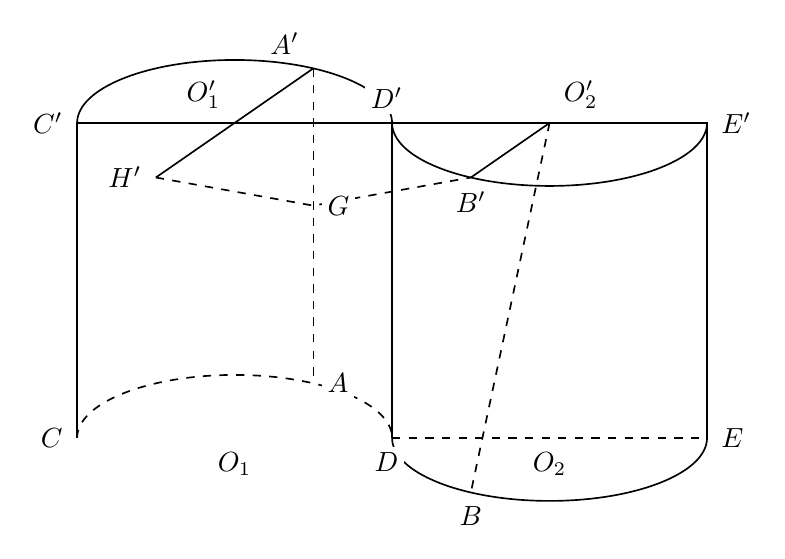
\begin{tikzpicture}[x=1cm,y=1cm,font=\normalsize,
  geometry edge/.style={draw=black,solid,line width=.6pt},
  geometry hidden/.style={draw=black,dashed,line width=.6pt},
  geometry label/.style={font=\normalsize,inner sep=2pt,fill=white}]
\coordinate (C) at (0.0,0.0);
\coordinate (D) at (4.0,0.0);
\coordinate (E) at (8.0,0.0);
\coordinate (Cp) at (0.0,4.0);
\coordinate (Dp) at (4.0,4.0);
\coordinate (Ep) at (8.0,4.0);
\coordinate (O1) at (2.0,0.0);
\coordinate (O1p) at (2.0,4.0);
\coordinate (O2) at (6.0,0.0);
\coordinate (O2p) at (6.0,4.0);
\coordinate (A) at (3.0000000000,0.6928203230);
\coordinate (Ap) at (3.0000000000,4.6928203230);
\coordinate (G) at (3.0000000000,2.9500000000);
\coordinate (Hp) at (1.0000000000,3.3071796770);
\coordinate (Bp) at (5.0000000000,3.3071796770);
\coordinate (B) at (5.0000000000,-0.6928203230);
% left box
\draw[geometry edge] (C)--(Cp)--(Ep)--(E);
\draw[geometry edge] (Cp) arc (180:0:2 and .8);
\draw[geometry hidden] (C) arc (180:0:2 and .8);
\draw[geometry edge] (Dp) arc (180:360:2 and .8);
\draw[geometry edge] (D) arc (180:360:2 and .8);
\draw[geometry hidden] (D)--(E);
\draw[geometry hidden] (Ap)--(A);
\draw[geometry edge] (Ap)--(Hp);
\draw[geometry hidden] (Hp)--(G)--(Bp);
\draw[geometry edge] (O2p)--(Bp);
\draw[geometry hidden] (O2p)--(B);
\draw[geometry edge] (Dp)--(D);
\node[geometry label,left,xshift=-3.0pt] at (Cp) {$C'$};
\node[geometry label,left,xshift=-3.0pt] at (C) {$C$};
\node[geometry label,above,xshift=-2.0pt,yshift=3pt] at (Dp) {$D'$};
\node[geometry label,below,xshift=-2.0pt,yshift=-3pt] at (D) {$D$};
\node[geometry label,right,xshift=3.0pt] at (Ep) {$E'$};
\node[geometry label,right,xshift=3.0pt] at (E) {$E$};
\node[geometry label,above left,xshift=-3pt,yshift=3pt] at (Ap) {$A'$};
\node[geometry label,right,xshift=3pt] at (A) {$A$};
\node[geometry label,right,xshift=3pt] at (G) {$G$};
\node[geometry label,left,xshift=-3pt] at (Hp) {$H'$};
\node[geometry label,below,yshift=-3pt] at (Bp) {$B'$};
\node[geometry label,below,yshift=-3pt] at (B) {$B$};
\node[geometry label,above left,xshift=-3pt,yshift=3pt] at (O1p) {$O_{1}'$};
\node[geometry label,below,yshift=-3pt] at (O1) {$O_{1}$};
\node[geometry label,above right,xshift=3pt,yshift=3pt] at (O2p) {$O_{2}'$};
\node[geometry label,below,yshift=-3pt] at (O2) {$O_{2}$};
\end{tikzpicture}